\documentclass[10pt,twocolumn,a4paper]{book}
\usepackage[unicode=true,
    pdfauthor={김세훈},
    pdftitle={SD와 HD 영상 측정 가이드},
    pdfsubject={Tektronix의 A guide to standard and high-definition digital video measurements를 번역한 문서},
    pdfkeywords={Television, Video},
    colorlinks=true,
    linkcolor=blue,
    citecolor=blue,
    anchorcolor=blue]{hyperref}

\usepackage[hangul]{kotex}
\usepackage{makeidx}
\usepackage{graphicx}
\graphicspath{{./images/}}

\usepackage{geometry}

	
\usepackage{fancyhdr}
\pagestyle{fancy}
\renewcommand{\headrulewidth}{0pt}
\fancyhead{} 
\fancyfoot{}
\fancyfoot[LE,RO]{\thepage}


\usepackage{silence}
\WarningsOff*


\usepackage{newfloat}
\DeclareFloatingEnvironment[name=표]{tab}

\usepackage{xcolor}
\usepackage{titlepic}
\usepackage{titlesec}


\usepackage{amsmath,amssymb}
\usepackage{IEEEtrantools}

\usepackage{chngcntr}
\counterwithout{figure}{chapter}
\counterwithout{tab}{chapter}

\usepackage[skip=0pt]{caption}

\usepackage{float}

\usepackage{pdfpages}

\usepackage{fontspec}
\hangulfontspec{Noto Sans KR}
\setmainhangulfont{Noto Sans KR}
\setsanshangulfont{Noto Sans KR}

\raggedbottom

\usepackage{tabu}

\makeatletter

\renewcommand{\thechapter}{}
\renewcommand\chapter{\if@openright\cleardoublepage\else\clearpage\fi
                    \thispagestyle{fancy}% original style: plain
                    \global\z@
                    \@afterindentfalse
                    \secdef\@chapter\@schapter}
\makeatother


\newcommand{\image}[5][width=\textwidth]{
    \begin{figure*}[#2]
        \centering
        \includegraphics[#1]{#3}
        \caption{#4}\label{#5}
    \end{figure*}
}
\AfterEndEnvironment{figure*}{\noindent\ignorespaces}

\newcommand{\himage}[5][width=0.48\textwidth]{
    \begin{figure}[#2]
        \centering
        \includegraphics[#1]{#3}
        \caption{#4}\label{#5}
    \end{figure}
}
\AfterEndEnvironment{figure}{\noindent\ignorespaces}

\newcommand{\tbl}[5][width=\textwidth]{
    \begin{tab*}[#2]
        \centering
        \includegraphics[#1]{#3}
        \caption{#4}\label{#5}
    \end{tab*}
}
\AfterEndEnvironment{tab*}{\noindent\ignorespaces}

\newcommand{\htbl}[5][width=0.48\textwidth]{
    \begin{tab}[#2]
        \centering
        \includegraphics[#1]{#3}
        \caption{#4}\label{#5}
    \end{tab}
}
\AfterEndEnvironment{tab}{\noindent\ignorespaces}

\setcounter{secnumdepth}{0}


\titleformat{\chapter}[display]
{\normalfont\bfseries}{}{0pt}{\Huge}

\hypersetup{pdfencoding=auto}

\makeindex

\begin{document}

\null
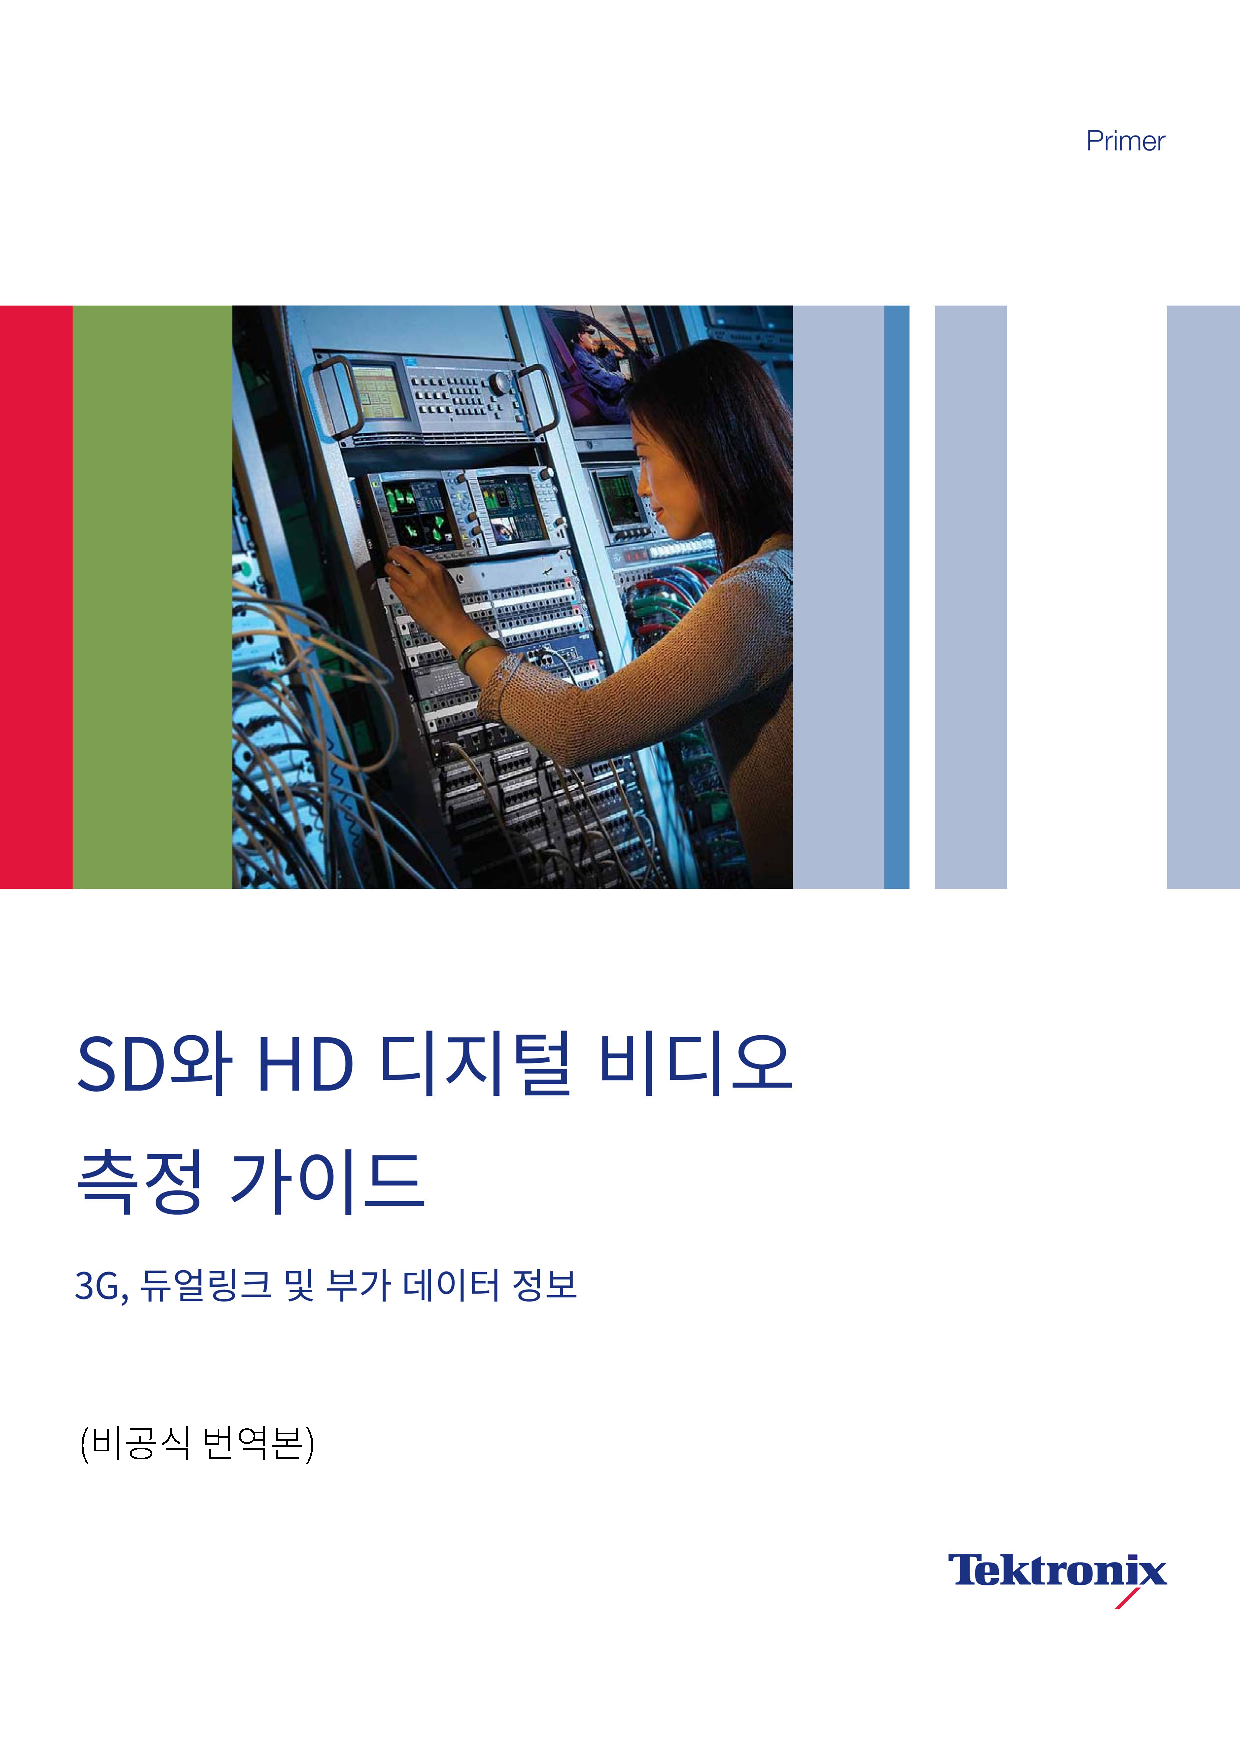
\includepdf[fitpaper=true]{표지.pdf}
\thispagestyle{empty}

\tableofcontents

\section{안내}
이 문서는 Tektronix 사의 허가 아래 SBS의 김세훈이 번역하였습니다. 모든 저작권은 Tektronix 사에서 설정한 바에 따릅니다.

\twocolumn
\chapter{시작}
디지털 텔레비전은 뭔가 매우 과학적이고 복잡한 것이라고 생각하기 쉽다. 하지만 최종 결과물은 친숙한 것이다.
그것은 바로 텔레비전 엔지니어들이 처음부터 계속 추구해온 것들, 즉 계속해서 좋아지는 시청 경험, 바로 아티스트의 퍼포먼스를 시청자들에게 더 잘 전달하는 양질의 비디오와 오디오이다.
디지털 텔레비전에서 유일하게 새로운 것은 정보(메시지)가 전달되는 방법 뿐이다.

메시지가 어떻게 전달되는지가 정말 중요할까? 아티스트와 시청자들(그리고 많은 나라에서 광고주들)은 신호가 전달되는 경로를 신경쓰지 않을 것이다.
그들은 디지털 텔레비전의 개선된 품질만을 누릴 뿐이지 자세한 것은 모른다. 하지만 이론, 바로 이것이 재미있는 부분이다.
텔레비전의 기술적인 부분에 관련있는 우리 엔지니어들은 이론에 신경을 쓰고, 지난 60년 이상의 시간 동안 크게 발전한 텔레비전 이론의 혜택을 누린다.
그 중에서 지난 20년간 디지털 텔레비전이 가져온 발전을 특히 더 누린다.

프로그램 영상, 디지털 오디오, 그리고 관련된 부가 데이터 신호들이 모여서 디지털 텔레비전 신호를 이룬다.
아날로그 텔레비전 세상에서는 비디오와 오디오는 완전히 분리된 경로를 통해 소스로부터 가정의 수상기로 전달된다.
디지털 신호들은 훨씬 더 자유롭게 비디오, 오디오 및 다른 신호들이 하나의 데이터 흐름으로 엮여서 구성될 수 있다.
우리가 알아야 할 것은 데이터가 어떻게 구성되어서 우리가 원하는 것을 어떻게 골라낼 수 있는지 뿐이다.

\section{전통적인 텔레비전}
아날로그 비디오와 아날로그 오디오를 전통적인 텔레비전의 요소라고 할 수 있을 것이다. 하지만 우리는 전통적인 목표를 이루기 위해, 어쩌면 더 많은 것을 이루기 위해 노력한다는 것을 알아야 한다.
디지털 텔레비전은 아날로그에 기반하고, 디지털 텔레비전에 대한 이해는 아날로그 텔레비전의 이해에서 나온다.
카메라 렌즈로 들어가는 빛과 마이크로 들어는 소리는 여전히 아날로그이다. 디스플레이에서 빛이 나오고 소리가 귀로 들어가는 것 역시 아날로그 현상이다.

우리는 이미 아날로그 비디오는 빛의 값을 샘플링한 것임을 알고 있다. 밝기 값은 전압으로 표현된다. 거기에 추가적인 정보가 샘플의 색상을 알려준다.
샘플들은 동기화된 상태로 전송 시스템 내에서 전달되어 디스플레이에서 원래 이미지를 다시 만들어내게 된다.
아날로그 비디오는 수상기가 적절히 처리하는 방법을 알면 그림을 다시 만들어낼 수 있는 데이터들을 담고 있는 전압값들의 직렬 흐름으로서 전달된다.
따라서 단순히 몇몇 단어만 바꾸고, 지난 50년간 배워온 것들을 이용하기 위해서 몇몇 가지만 다르게 하면 디지털 비디오는 아날로그 비디오와 그리 다르지 않음을 알 수 있다.

그럼, 아날로그 빛에서 시작해서 아날로그 빛으로 끝난다면 디지털 비디오를 도대체 왜 쓰는 것일까?
많은 경우, 카메라 센서는 아날로그 비디오를 만들어내지만, 거의 즉시 순간순간의 영상의 값을 나타내며 변동하는 아날로그 전압값을 디지털로 바꿔서 근본적으로 열화 없이 다룰 수 있게 한다.
컴퓨터 그래픽과 같은 몇몇 경우에는 비디오가 디지털로 시작하며, 최신의 디지털 텔레비전 시스템 내에서는 아날로그로 변환되지 않고 디스플레이로 도달한다.

우리는 텔레비전 신호를 여전히 아날로그 NTSC, PAL, SECAM 전송 방식으로 보낼 수 있지만, 더 높은 품질과 더 높은 효율로 텔레비전 신호를 보내기 위해서 디지털 전송을 하고 있다.
디지털 텔레비전은 일상 생활내에서 누릴 수 있는 일부가 되었다. 누군가는 이를 이용하며 발전에 기여할 것이고, 누군가는 세부사항을 모른 채 혜택을 누릴 것이다.
\chapter{새로운 디지털 텔레비전}
디지털 신호는 몇 년간 텔레비전의 일부가 되어왔는데, 처음에는 테스트 신호와 자막 생성기 같은 장비 내에서 보이지 않게 묻혀있다가, 나중에는 전체 시스템으로 퍼졌다.
이 글에서는 쉽게 접근하기 위해 우선 텔레비전 신호의 비디오 부분을 다룰 것이다.
오디오 또한 마찬가지로 디지털일 것이고, 디지털 데이터가 복원되는 텔레비전 수상기에서 재생될 것이다. 디지털 오디오는 뒤의 장들에서 다뤄질 것이다.
\\
디지털 비디오는 아날로그 비디오의 간단한 확장이다. 한번 아날로그 비디오를 이해하고 나면, 디지털 비디오가 어떻게 만들어져서 다뤄지고, 처리되고, 아날로그 신호와 어떻게 상호 변환되는지 이해하기 쉽다.
아날로그와 디지털 비디오에는 많인 비슷한 제약 조건들이 있고, 디지털 영역에서 발생할 수 있는 많은 문제들은 나쁜 아날로그 소스 비디오에 기인한다.
따라서, 아날로그와 디지털 비디오 장치의 설계와 작동에 대한 기준이 되는 표준을 마련하는 것이 중요하다.

\section{아날로그 세계를 설명하는 숫자들}
초기 디지털 비디오는 단순히 아날로그 NTSC나 PAL 컴포지트 비디오 신호의 디지털 표현일 뿐이었다.
표준들은 작동 한계를 설명하고 각 전압 레벨을 설명하는 숫자들과 각 숫자들이 어떻게 만들어지고 복원되는지를 규정했다.
데이터 속도가 빨랐기 때문에 디지털 비디오 데이터를 내부적으로 8비트나 10비트 버스로 다루는 게 일반적이었고, 초기 표준들은 여러 선을 이용한 외부 연결을 다뤘다.
표준들은 수상기와 전달된 데이터들을 동기화하고 또 임베디드 오디오와 같은 추가적인 기능을 제공하는 특정한 부가 데이터와 관리 데이터들을 설명했다.
나중에, 고속 처리가 가능해지자, 단일 선을 이용한 직렬 인터페이스 표준이 만들어졌다.
기본적으로, 디지털 비디오는 아날로그 전압의 숫자 표현이며, 빠르게 변하는 비디오와 필요한 부가 데이터를 담기 충분하게 빠르게 나타나는 숫자 데이터들이다.

\section{컴포넌트 디지털 비디오}
초기 아날로그 효과 장치 설계자들은 빨강, 초록, 파랑 채널을 신호처리 과정에서 최대한 분리하는 것의 이점을 깨달았다.
NTSC와 PAL 인코딩/디코딩 과정은 투명하지 않으므로(역주: 정보를 그대로 보존하지 않으므로) 여러 번 인코딩하고 디코딩하는 것은 점점 신호를 열화시킨다.
카메라 신호는 빨강, 초록, 파랑 각각의 독립적인 정보에서 시작하고, 이 신호들을 시스템 내에서 최대한 덜 포맷 변환을 해서 NTSC나 PAL 신호로 인코딩해서 시청자들에게 보내는 게 가장 좋다.
하지만 이 세 개의 서로 관련있는 정보의 채널을 개별적으로 방송국 내에서 다루는 것은 물류 문제(역주: 케이블 포설 등)와 신뢰성 문제를 일으킨다.
실질적인 관점에서, 이 세 신호는 하나의 선 혹은 동축 케이블 내에 같이 존재해야 한다.
이 세 가지 빨강, 초록, 파랑 비디오 채널들을 행렬을 이용하여 섞어서 보다 효율적인 휘도와 두 가지 색차 신호로 만들어서 각각을 디지털화한 후 하나의 동축 케이블에 다중화해서 담으면 되는 것으로 밝혀졌다.
이 데이터 신호를 NTSC나 PAL 컴포지트 비디오 다루듯이 다룰 수 있다. 이제 우리는 고속의 숫자 데이터 흐름을 다루고 있다.
이 데이터 신호는 NTSC나 PAL 비디오 신호의 5~6 MHz 신호보다 훨씬 빨리 변하는 에너지를 담고 있지만, 어느 정도 실질적인 거리까지는 손실 없이, 별다른 조치 없이 다룰 수 있다.
한번 비디오 신호가 디지털 영역으로 들어오면, 우리는 디지털 영역 내에서 추가적인 손실이나 채널 간 영향 없이 각 구성 요소들을 뽑아서 개별적으로 처리하고 다시 합칠 수 있다.
\\
각 요소와 디지털 기술은 비디오 품질 관리에 큰 도움을 주었으며, 디지털 장치들의 속도는 HD 비디오의 대역폭을 실현 가능하게 했다.
디지털은 필요한 데이터량을 줄일 수 있게 해주는 다양한 압축 알고리즘을 이용한 처리가 가능하게 한다.
이제 HD 비디오와 다채널 오디오를 고품질 실시간 아날로그 비디오에서 요구되는 대역폭 내에서 전송할 수 있다.
비디오 압축이라는 주제는 많은 출판물에서 다뤄지고 있으며(참고 문헌을 보라) 이 글에서는 다루지 않을 것이다.
\chapter{아날로그에서 디지털로}

디지털 데이터 스트림은 각각의 개별 구성 요소들로 쉽게 분해될 수 있는데, 이들은 보통 아날로그에서 대응되는 것들과 같은 역할을 한다.
아날로그와 디지털 비디오 영역을 설명하고 비교하는 동안 계속 이 관계를 사용할 것이다.
한번 아날로그와 디지털 비디오의 유사성을 이해하고 나면 HDTV를 다룰 수 있는데, 보통 이는 이에 대응되는 HD 아날로그 포맷의 디지털적 표현이다.


NTSC와 PAL 비디오 신호들은 색의 삼원색인 빨강, 초록, 파랑 세 개의 카메라 채널의 합성인데, 행렬을 이용하여 합쳐져서 휘도를 만들고 이는 두 개의 색상 정보를 담고 있는 반송파 억압 변조 신호와 합쳐진다.
세 번쨰 단일 채널 컴포지트 전송 시스템은 SECAM 시스템인데, 이는 색상 정보를 전달하기 위해 한 쌍의 주파수 변조된 부반송파들을 이용한다.
스튜디오에서의 카메라의 RGB 감지 장치와 종단 디스플레이의 RGB 채널 사이의 어느 단에서도 신호가 특별히 NTSC, PAL 혹은 SECAM이 될 필요는 없다.
NTSC, PAL 또는 SECAM에 대한 이해로 충분한 이상, 컴포지트 비디오에 대해서 더 많은 이해를 추구하진 않겠다.

\section{RGB 컴포넌트 신호}
\image{h!}{rgb camera to monitor direct.pdf}{카메라에서 모니터까지의 RGB 직결 연결}{fig1 rgb camera to monitor direct}
\image{h!}{video encodeded into ntsc pal.pdf}{단일 동축 케이블 전송을 위해 NTSC 또는 PAL로 인코딩된 비디오}{fig2 video encodeded into ntsc pal}
\image{h!}{digital no degradation.pdf}{디지털 전송에서는 아날로그적 신호 열화가 발생하지 않는다}{fig3 digital no degradation}
비디오 카메라는 이미지를 빛의 삼원색인 빨강, 초록, 파랑으로 분해한다. 카메라의 센서들은 이 각각의 단색 이미지들을 각각의 전기 신호로 변환한다.
화상의 왼쪽 끝과 최상단을 알려주는 동기 정보가 이 신호들에 추가된다. 디스플레이를 카메라와 동기화시키는 정보가 초록 채널에, 때로는 모든 채널에 더해지거나 아니면 별도로 전달된다.


가장 간단한 배선은 \figurename~\ref{fig1 rgb camera to monitor direct}에 나와 있듯이 R, G, B를 카메라에서 그대로 받아서 모니터에 연결하는 것이다. 여러 선을 이용한 전송 시스템은 아날로그 SD든 아날로그 HD든 구조가 같다.
여러 선을 이용한 연결은 작고 영구적으로 변경되지 않도록 구성된 하위 시스템에서 사용될 수 있을 것이다.


이 방법은 카메라에서 디스플레이까지 고품질의 이미지를 만들어내지만, 신호를 세 분리된 채널로 전송하기 위해선 엔지니어가 각 채널이 신호를 처리할 때 같은 이득, 직류 오프셋, 시간 딜레이와 주파수 응답을 갖게 해야 한다.
각 채널의 이득이 다르거나 직류 오프셋에 오차가 생기면 최종 디스플레이 출력에서 미묘한 색상 변화가 일어날 것이다.
시스템에 타이밍 오차가 있을 수도 있는데, 이는 케이블 길이가 다르거나 각 신호를 카메라에서 디스플레이까지 라우팅하는 경로가 달라서 생길 수 있다.
이는 채널간 타이밍 오프셋을 만들 것이고 영상이 뭉개지게 만들 것이고, 심한 경우 이미지가 분리되어 여러 개가 나타날 것이다.
주파수 응답의 차이는 채널이 합쳐질 때 일시적인 악영향을 만들 것이다.
분명히 세 채널을 하나로 다룰 방법이 필요하다.


NTSC나 PAL 인코더와 디코더를 \figurename~\ref{fig2 video encodeded into ntsc pal}\와 같이 추가하는 것은 방송국 내에서 신호가 하나의 선으로 다뤄지는 것 외에는 단순화에 도움을 주지 못한다.
시스템 대역폭은 세 비디오 신호의 에너지를 4.2 MHz(NTSC)나 5.0에서 5.5 MHz(PAL) 내에서 다루기 적절하게 정해진다.
단일 선 구성은 비디오 라우팅을 쉽게 해 주지만, 더 먼 경로에 대해서 주파수 응답과 타이밍 문제를 고려해야 한다.
NTSC와 PAL 신호 모두에서 색상차와 휘도는 4.2 MHz(NTSC) 또는 5.0에서 5.5 MHz(PAL)의 대역폭을 공유하므로, 여러 번의 인코딩과 디코딩은 피해야 한다.
(역주: 좁은 대역폭 안에 신호가 들어가므로 열화를 피해야 함)


위의 시스템에서 NTSC/PAL 인코더와 디코더를 컴포넌트 디지털 인코더와 디코더로 대체함으로써 \figurename~\ref{fig3 digital no degradation}의 구성은 더 복잡하지도 않으면서 더 좋은 성능을 보인다.
하나의 동축 케이블에 들어있는 에너지는 SD 신호일 경우 270 Mb/s, HD 신호일 경우 1.485 Gb/s 이상의 속도이다.
SD 신호는 전통적인 방송 텔레비전 채널을 통한 전송을 하기 위해 아날로그 NTSC나 PAL로 변환될 수 있다.
HD 신호는 기존의 NTSC나 PAL 채널의 대역폭에 맞춰져서 공중파로 전송되기 위해서 압축되어야 한다.

\image{h!}{bt 709 gamma.pdf}{BT.709 감마 보정은 CRT 디스플레이의 응답을 보정한다}{fig4 bt 709 gamma}
\section{감마 보정}
비디오 신호를 다룰 때 고려해야 할 아날로그 요소는 비디오 디스플레이는 장면의 각 요소들의 밝기를 정확하게 표현한다고 인식되는 점이다.
음극선관(CRT) 디스플레이는 근본적으로 비선형 장치로서, 디스플레이에 가해지는 전압은 비선형적인 함수에 따라 정해지는 빛의 양으로 출력된다.
이 함수가 장치의 감마이다. 선형적인 응답을 얻기 위해서 TV 시스템 내에서 보정이 가해져야 한다.
따라서, 카메라의 RGB 신호는 CRT의 응답의 역함수에 의한 감마 보정이 이루어진다. 감마 보정된 신호는 R', G', B'와 같이 프라임(')마크가 붙어서 감지 장치에서 디스플레이로의 전달 함수에 대한 보정이 들어갔음을 나타낸다.
프라임 마크가 귀찮고, 때로 부적절하게 생략되긴 하지만, 이 글에서는 표준 문서를 따라 계속 사용될 것이다.


LCD와 PDP가 보편적인 오늘날에는(역주: 이 글이 처음 쓰인 지 꽤 시간이 지났다) 감마 보정이 더 이상 필요 없을 것이라고 생각될 수도 있다.
하지만, 인간의 밝기에 대한 시각 반응도 지수함수적인데, 약 1/3승을 따른다. 가장 좋은 명암 표현과 신호대잡음비(S/N, SNR)를 위해서 비디오 인코딩은 같은 지수함수를 이용한다. 이를 인지적 코딩이라고 한다.

\section{감마 보정은 CRT 반응에 대한 보정 이상을 의미한다}
CRT를 위한 감마 보정은 거의 최적의 인지적 보정이다. 이러한 이유로, 감마 보정 장치가 있는 시스템을 평가할 때는 유의해야 한다.


\figurename~\ref{fig4 bt 709 gamma}\는 디지털 HD 비디오에 대해 널리 사용되는 ITU-R BT.709 표준에 따른 0.45제곱을 이용한 감마 보정을 보여준다.
이 감마 보정은 CRT의 비선형성 교정과 인지적 코딩을 위해서 카메라에 적용된다. CRT의 비선형성은 2.2에서 2.6의 지수를 갖는 지수함수이고, 대부분의 CRT는 2.5의 지수를 갖는다.
최종적인 전체 시스템의 감마는 약 1.2(역주: $0.45\times 2.5\approx 1.2$)로 일반적인 시청 환경에서 거의 이상적인 값이다. 이 응답은 대략적으로 인간의 밝기 인지 특성에 적합하고, 결과적으로 비디오가 전송을 위해 디지털화될 때에 필요한 비트 수를 줄여준다.

\tbl{h!}{luma and chroma components.pdf}{휘도와 색상 비디오 요소}{table1 luma and chroma components}
\htbl{h!}{luma and chroma for composite encoding.pdf}{컴포지트 비디오 인코딩을 위한 휘도와 색차 값}{table2 luma and chroma for composite encoding}
\section{R'G'B'신호의 휘도와 색상차 신호로의 변환}
빨강, 초록, 파랑의 RGB 비디오 요소들은 카메라의 감지 장치의 근본적인 것들이고 비디오 색상을 다룰 때 거의 항상 이용된다.
하지만 RGB는 비디오 처리를 할 때 이미지를 전달하는 가장 대역폭 효율적인 방법은 아닌데, 이는 세 신호가 모두 같은 대역폭을 가져야 하기 때문이다.
인간의 시각은 색의 변화보다 밝기의 변화에 더 민감하므로 이를 이용해서 최대 대역폭의 휘도 신호와 남는 대역폭을 차지하는 색차 신호들을 끌어냄으로써 대역폭 효율을 향상시킬 수 있다.


비디오 신호 요소들을 휘도와 색차 값으로 처리하는 것은 전달되어야 하는 정보량을 줄여준다. 밝기와 신호의 세부 표현을 담당하는 휘도 채널(Y')에 전체 대역폭을 할당함으로써, 두 개의 색차 채널(R'-Y'와 B'-Y')은 휘도 채널 대역폭의 절반 정도만 사용해도 충분한 색 정보를 제공할 수 있다.
이를 이용해서 간단한 선형 행렬로 R'G'B'와 Y',R'-Y',B'-Y'를 상호 변환할 수 있다. 색차 신호 채널의 대역폭 제한은 행렬 연산 이후에 시행된다.
채널이 디스플레이에서 R'G'B'로 복원될 때, 밝기 세부 정보는 전체 대역폭을 이용해서 복원되고 공간적인 색 세부 정보는 받아들일 만한 정도로 제한된다.
다음에 나오는 문단과 표에서 인코더와 디코더 내에서 일어나는 R'G"B'에서 Y',R'-Y', B'-Y'로의 변환을 다룰 것이다.


감마 보정된 R'G'B' 요소들은 행렬을 이용해서 감마 보정된 휘도(Y')와 두 개의 색차 요소로 바뀐다. 휘도와 색차 요소들은 표 \ref{table1 luma and chroma components}에 나온 값들을 이용해서 R',G',B'로부터 나온다(각 계수들의 단위는 볼트이다).


표 \ref{table1 luma and chroma components}\은 R'G'B'에서 Y',(R'-Y'),(B'-Y')로의 변환에 사용되는 전압의 범위를 알려준다. 휘도 신호는 0에서 700 mV의 다이내믹 레인지를 갖는다.
색차 신호들인 R'-Y'와 B'-Y'는 여러 컴포넌트 포맷들에 따라 달라지는 배율에 의해 다른 다이내믹 레인지를 가질 수 있다. Y'P'bP'r로 표기되는 아날로그 요소 포맷에서는 두 색차 값은 $\pm 350$ mV의 다이내믹 레인지를 갖는다. 이는 비디오 신호 처리를 더 단순하게 해준다.
아날로그 Y'Pb'Pr' 값은 디지털 표준에서 보통 사용되는 Y'C'bC'r을 만들기 위한 오프셋 역할을 한다. 이로부터 나오는 비디오 요소들은 흑백 비디오 신호와 비슷한 Y' 또는 휘도 채널과 두 개의 색차 채널인 C'b와 C'r인데 이들은 밝기 정보 없이 색상 정보만 전달하며 이 세 신호는 모두 디지털 데이터로 양자화되기 쉽게 적절하게 배율이 곱해진다.


여러 다른 색차 포맷들이 다양한 응용(목적)에서 사용된다. 컴포지트 PAL, SECAM과 NTSC 인코딩에서 현재 사용되는 배율 값들이 표 \ref{table2 luma and chroma for composite encoding}에 나와 있는 것처럼 다르다는 것을 아는 것은 특히 중요하다.

\chapter{디지털 비디오 인터페이스}
\image{!t}{digitizing rgb camera.pdf}{RGB 카메라 신호의 디지털화}{fig:digitizing rgb camera}
이 시점에서 아날로그 비디오와 연결하는 디지털 인터페이스를 간단히 살펴보는 게 적절하다.
\figurename~\ref{fig:digitizing rgb camera}부터 \figurename~\ref{fig:recovering analog values from prallel data}까지의 블록 다이어그램은 비디오 프로덕션 장비가 디지털 비디오 요소들을 어떻게 다루는지 이해하는 데 도움을 줄 것이다.
이 그림들이 SD 시스템을 다루긴 하지만, 기본 개념은 HD 포맷에서도 똑같다. HD 포맷에서는 샘플링과 데이터 속도가 더 빠르고 각각 분리된 10비트의 휘도와 색차 버스가 시스템 전체에서 더 유지되고, 이를 통해서 고속으로 작동해야 하는 회로를 줄인다.
\\
감마 보정된 RGB(\figurename~\ref{fig:digitizing rgb camera})는 선형 행렬을 통해서 휘도 요소인 Y'과 두 개의 배율이 곱해진 색차 요소인 P'b와 P'r로 바뀐다.
눈은 색상 변화보다 밝기 세부 정보의 변화에 더 민감하므로, Y'신호는 시스템 내에서 더 높은 대역폭으로 전달된다(SD의 경우 5.5 MHz).
휘도와 색차 신호는 샘플링(디지털화) 과정에서 에일리어싱을 일으킬 수 있는 고주파 비디오 성분을 제거하기 위해서 저역 통과 필터로 처리된다.
필터링된 휘도 신호는 아날로그-디지털 변환기에서 13.5 MHz의 속도로 샘플링되어 13.5 Mb/s의 10비트 데이터 스트림으로 바뀐다.
두 개의 색차 신채널들은 필터링된 후 아날로그-디지털 변환기에서 6.75 MHz의의 속도로 2개의 6.75 Mb/s의 데이터 스트림으로 바뀐다.
세 비디오 채널들은 27 Jb/s의 단일 10비트 병렬 데이터 스트림으로 다중화되어 합쳐진다.
\image{h!}{processing and serializing parallel data stream.pdf}{병렬 데이터 스트림의 처리와 직렬화}{fig:processing and serializing parallel data stream}
보조 처리기(\figurename~\ref{fig:processing and serializing parallel data stream})가 타이밍 기준 신호, AES/EBU 포맷의 디지털 오디오와 기타 부가 데이터를 추가한다. 데이터에 대한 체크섬 또한 계산되어서 병렬 데이터 스트림에 추가된다.
\\
27 Mb/s, 10 비트의 병렬 데이터는 270 Mb/s로 작동하는 시프트 레지스터(또는 직렬화기)로 입력되어서, 이 예제에서는 SD 표준인 ITU-R BT-656/SMPTE 259M을 따르는 적절한 전송을 위해서 스크램블된다.
\\
SD ITU-R BT-656/SMPTE 259M 적합 신호는 표준 비디오 케이블을 따라서 거의 100\%의 무결성을 유지하며 300 m를 갈 수 있다. 1.485 Gb/s의 HD SMPTE 292M 적합 신호는 약 100 m를 갈 수 있다.
\image{!t}{sdi receiver.pdf}{SDI 수신기 - 비디오 데이터를 역직렬화하여 다시 병렬로 만든다}{fig:sdi receiver}
수상기에서는(\figurename~\ref{fig:sdi receiver}) 절반 클럭 주파수의 에너지가 감지되어서 270 Mb/s로 입력되는 신호를 적절히 아날로그 등화 처리한다. 새로운 270 MHz 클럭이 NRZI(Non-Return to Zero Inverse) 신호의 에지에서 복원되고, 등화된 신호가 논리 상태를 결정하기 위해서 샘플된다.
역직렬화기는 인코더의 스크램블 알고리즘의 역변환을 이용해서 스크램블을 해제하여 27 Mb/s의 10비트 데이터 스트림을 만든다. 임베디드된 체크섬이 수신기에서 추출되어서 수신된 데이터로부터 새로 계산된 체크섬과 비교되어 오류가 발생했는지 확인하고 적절한 플래그를 데이터 스트림에 붙인다.
보조 처리기는 오디오나 다른 부가 데이터들을 추출한다.
\image{!t}{recovering r'g'b' from parallel data.pdf}{병렬 데이터에서 아날로그 R'G'B'를 복원}{fig:recovering analog values from prallel data}
10비트 데이터 스트림은 역다중화되어(\figurename~\ref{fig:recovering analog values from prallel data}) 디지털 휘도와 색차 스트림이 되고, 3개의 디지털-아날로그 변환기를 통하여 아날로그 신호가 되며, 이산적인 데이터 레벨에서 부드러운 아날로그 신호가 되도록 (역자 주:저역) 필터를 통과하고 디스플레이에서 원래의 R'G'B'신호가 되게 행렬을 이용해서 합쳐진다.
\\
이 간단한 시스템 개관은 시스템이 어떻게 작동하는지 이해하는 데 도움이 될 것이다. 추가적인 디지털 인터페이스에 대한 세부적인 설명은 뒤의 문단들에서 나올 것이다.

\section{601 샘플링}
\image{t!}{color difference quantizing.pdf}{색차 신호의 양자화}{fig:color difference quantizing}
\image{h!}{luminance quantizing.pdf}{휘도 신호의 양자화}{fig:luminance quantizing}
ITU-R BT.601은 625/50과 525/60 텔레비전 시스템의 디지털 요소들에 대한 파라미터를 결정하기 위한 연합 SMPTE/EBU 태스크 포스에서 만들어진 샘플링 표준이다.
이 작업은 1981년에 SMPTE에 의해 후원된 일련의 테스트들로 완결되었고, 잘 알려진 CCIR 권고안 601 (이제는 ITU-R BT.601)이라는 결과가 나왔다.
이 표준 문서는 525와 625줄 신호에서 사용되는 샘플링 방법을 규정한다. 이는 아날로그 휘도에 대한 13.5 MHz와 두 개의 아날로그 색상차 신호에 대한 6.75 MHz의 직교 샘플링을 규정하고 있다.
샘플링된 값들은 디지털 휘도인 Y'와 디지털 색차 신호인 C'B와 C'r인데 이들은 아날로그의 감마 보정 신호인 B'-Y'와 R'-Y'에 배율이 곱해진 것이다.
525줄과 625줄 시스템에서 공통적인 요소인 2.25 MHz가 13.5 MHz의 약수이기 때문에 13.5 MHz라는 샘플링 주파수가 선정되었다(부록 B - 텔레비전 클럭 관계를 참고하라).
\\
현재 많은 ITU-R BT.601 구현들이 10 비트 샘플링을 쓰고 있지만, ITU-R BT.601은 8비트 샘플링($00_h$부터 $FF_h$까지 256레벨을 갖는)과 10비트 샘플링($000_h$부터 $3FF_h$까지 1024 레벨을 갖는) 모두를 허용한다.
8비트 워드는 바로 10비트로 변환될 수 있고, 10비트 값은 8비트 시스템과의 상호 운용성을 위해 8비트로 반올림된다. 색차 성분 C'r과 C'b 값들은 $\pm 350$ mV에 대응되는 $040_h$부터 $3C0_h$까지의 값을 갖는다.
이 범위를 넘어서는 신호도 허용되고, 최종적으로 가능한 범위는 $\pm 400$ mV이다. 휘도 성분 Y' (\figurename~\ref{fig:luminance quantizing})의 값의 범위는 $040_h$부터 $3AC_h$의 값을 갖는데 이는 아날로그 신호의 0.0 mV부터 700 mV까지에 대응된다.
이 범위를 벗어나는 신호도 마찬가지로 허용되고, 흰색 레벨을 넘어서는 과한 값을 처리할 수 있는 더 넓은 여유 공간을 위해 최종적인 범위는 -48 mV부터 +763 mV까지가 된다.
아날로그/디지털 변환기들은 $000_h$부터 $003_h$와 $3FC_h$부터 $3FF_h$의 10비트 값을 생성하지 않도록 설정되는데 이는 8비트 시스템과의 상호 운용성을 위해서이다.
양자화 레벨은 8비트 레벨에 두 개의 0을 붙이면 10비트 값과 같은 값이 되도록 선택된다. 휘도와 색차 아날로그/디지털 컨버터 모두에서 $000_h$부터 $003_h$와 $3FC_h$부터 $3FF_h$까지의 값은 동기화를 위해 예약되어 있다.
\\
\himage{!h}{digital horizontal blanking interval.pdf}{디지털 수평 블랭킹 구간}{fig:digital horizontal blanking interval}
\image{!t}{layout of 2 to 1 interlaced digital frame.pdf}{2:1 비월 주사 디지털 프레임의 구조}{fig:layout of 2:1 interlaced digital frame}
\figurename~\ref{fig:digital horizontal blanking interval}\은 아날로그 수평 선에 대응되는 샘플들과 디지털 워드들의 위치를 보여주고 \figurename~\ref{fig:layout of 2:1 interlaced digital frame}\은 그림 영역과의 공간적인 관계를 보여준다.
타이밍 정보는 활성 비디오의 끝(EAV;End of Active Video)와 활성 비디오의 시작(SAV;Start of Active Video) 패킷이 전달하기 때문에 전통적인 동기화 신호는 필요하지 않다.
수평 블랭킹 구간과, 수직 블랭킹 구간의 전체 선 구간동은 오디오나 기타 부가 데이터를 전달하는 데 쓰일 수 있다. EAV와 SAV 타이밍 패킷은 데이터 스트림에서 $3FF_h, 000_h, 000_h$라는 워드로 시작하는 헤더로부터 알아낼 수 있다.
\\
"xyz"워드는 8비트 신호 경로에서 문제 없이 전달될 수 있게 2개의 가장 중요하지 않은 비트(역주: 끝의 2비트)가 0으로 설정된 10비트 워드이다.
SD에서 "xyz"워드들은 F ,V ,H라는 함수를 담고 있는데, 각 함수들은 다음의 값을 갖는다:
\begin{itemize}
    \item 8번째 비트 - (F비트) 첫 번째 필드에서 0, 두 번쨰 필드에서 1
    \item 7번째 비트 - (V비트) 수직 블랭킹 구간에서 1, 활성 비디오 선에서 0
    \item 6번째 비트 - (H비트) 1은 EAV 시퀀스를 가리키며 0은 SAV 시퀀스를 가리킴
\end{itemize}

\section{병렬 디지털 인터페이스}
Rec.601 샘플링에 의해 생성된 데이터의 전기적 인터페이스는 525/59.94를 위한 SMPTE 125M 표준과 625/50을 위한 EBU Tech. 3267로 별도로 표준화되었다. 두 표준 모두 CCIR(현 ITU)가 채택했고 병렬 하드웨어 인터페이스를 설명하는 권고안 656에 포함되었다.
병렬 인터페이스는 11개의 꼬인 쌍과 25개의 D 커넥터를 이용한다. 병렬 인터페이스는 데이터 워드들을 다중화하여 27 Mb/s의 속도의 C'b, Y', C'r, Y, ...의 시퀀스로 만든다. 타이밍 시퀀스인 SAV와 EAV가 각 선에 추가된다.
525와 625 포맷 모두의 디지털 활성 비디오 선은 720개의 휘도 샘플을 포함하는데, 남는 샘플들은 아날로그 블랭킹에 해당하며 타이밍과 기타 데이터에 이용될 수 있다.
\\
여러 전선과 패치 패널을 이용해야 하기 때문에, 디지털 스튜디오 장비들을 병렬로 연결하는 것은 작고 영구적으로 구성된 시스템에서만 현실적으로 이용할 수 있다.

\section{직렬 디지털 인터페이스(SDI)}
포맷과 상관없이 하나의 동축 케이블만으로 데이터를 보낼 필요가 분명히 있다. 이는 데이터 속도가 비교작 높아서뿐만이 아니라 신호가 적절히 변형되지 않으면 신뢰성 있는 복구가 어렵기 떄문이다(역주: 동기화가 필요하다).
신호는 전송 전에 신뢰성 있는 클럭 복구가 가능하게 충분히 많은 에지를 포함하고, 전송된 신호에 저주파 성분이 최소화되게 하고(역주: 시스템의 각 단은 보통 커패시터로 커플링되므로), 에너지 스펙트럼이 골고루 퍼져서 RF 방출 문제가 최소화되도록 변형되어야 한다.
스크램블링과 NRZI로의 변환을 이용하는 직렬 디지털 인터페이스가 이러한 요구사항을 만족시키기 위해 개발되었다. 이 시리얼 인터페이스는 ANSI/SMPTE 259M, ITU-R BT.656과 EBU Tech. 3267에 규정되어 있는데, SD 컴포넌트와 임베디드된 디지털 오디오를 포함하는 컴포지트 신호 모두에 대한 것이다.
이 직렬 인터페이스의 확대된 버전이 HD 전송을 위해서 규정되어 있다.

\himage{!h}{the carrier concept.pdf}{반송파 개념}{fig:the carrier concept}
개념적으로, 직렬 디지털 인터페이스는 스튜디오에서 응용되는 반송파 시스템과 유사하다. 기저대역 비디오와 오디오 신호는 디지털화되고 \figurename~\ref{fig:the carrier concept}에서 보여지는 것처럼 직렬 디지털 반송파 위에서 합쳐진다.
이 신호는 기저대역 디지털 신호이지 반송파 위에 변조된 게 아니라는 점에서 엄격히는 반송파 시스템이 아님을 명심하라.
비트율(반송파 주파수)는 디지털 데이터의 클럭으로 정해지는데, SD 컴포넌트 디지털에 대해서는 270 Mb/s이고 HD에 대해서는 1.485 Gb/s(또는 2.97 Gb/s)이다. (NTSC와 PAL 컴포지트 직렬 인터페이스의 143 Mb/s와 177 Mb/s 등 다른 속도도 사용되지만 여기서 자세히 다루지는 않겠다.)
\himage{!h}{parallel to serial conversion.pdf}{병렬에서 직렬로 변환}{fig:parallel to serial conv}

아날로그 신호 성분들을 표현하는 병렬 데이터는 \figurename~\ref{fig:parallel to serial conv}\와 같이 처리되어 디지털 데이터 스트림이 된다. 병렬용 클럭이 샘플 데이터들이 시프트 레지스터로 입력되는 데에 사용되고, 병렬용 클럭의 10배의 클럭이 각 10비트 워드들에 대해 LSB를 가장 먼저로 하여 비트들을 출력한다.
8비트 데이터만 가능하다면 직렬화기는 두 개의 LSB에 0을 채워서 10비트 워드를 완성한다. 컴포넌트 포맷에서는 병렬 인터페이스의 EAV와 SAV 타이밍 신호가 유일한 시퀀스를 만들어서 직렬 영역에서 이들을 이용해서 워드들을 프레임 단위로 만들 수 있게 한다.
EAV와 SAV 데이터 패킷을 코딩하는 방법은 이 글의 디지털 스튜디오 동기화 및 타이밍 장에 설명되어 있다. 오디오와 같은 다른 부가 데이터가 병렬 신호에 삽입되어 있다면, 이 데이터 또한 직렬 인터페이스에 의해 전달될 것이다.
\himage{!h}{nrz and nrzi.pdf}{NRZ와 NRZI의 관계}{fig:nrz and nrzi}

병렬 정보의 직렬화 뒤에는 데이터 스트림이 수학적 알고리즘에 의해 스크램블되고, 그 후에는 다음의 두 함수의 합성에 의해 NRZI로 인코딩된다.
\begin{IEEEeqnarray*}{lCr}
    G_1(X)=X^9+X^4+1$$\\
    G_2(X)=X+1$$
\end{IEEEeqnarray*}
스크램블링을 하면 통계적으로 신호가 적은 직류 성분을 갖게 되고 이는 신호를 다루기 쉽게 만든다. 또한 많은 상태 전환을 만들어내는데 이로부터 클럭 복구가 용이해진다. NRZI 포매팅은 신호의 극성이 중요하지 않게 만들어준다.
\\
수상기에서 역직렬화기는 이 알고리즘의 역 알고리즘을 이용해서 올바른 데이터를 복원해서 최종 시청자가 원래의 스크램블되지 않은 화면을 보게 해준다. 직렬 디지털 전송 시스템에서는 클럭이 별도 선으로 전달되는 병렬 시스템에서와는 달리 데이터 내에 클럭이 들어있다.
데이터를 스크램블링함으로써, 클럭 복원에 필요한 많은 상태 변환이 보장된다. 시스템의 스트레스 테스트를 위해서(디지털 시스템 테스팅 장을 보라) 높은 직렬 성분과 최소한의 상태 전환으로 이루어진 시퀀스를 갖는 신호가 특별히 고안되어서 SDI 수상기 회로의 성능을 테스트하는 데에 이용된다.
일반적으로 작동하는 직렬 디지털 시스템은 이러한 까다로운 신호에 대해서도 작동할 것이다.
\\
NRZI로 인코딩하는 것은 직렬 데이터가 극성에 민감하지 않도록 해준다. NRZ(Non-Return to Zero)는 친숙한 로직 레벨인 하이="1", 로우="0"을 이용한다. 전송 시스템에서는 수상기가 신호의 특정한 극성에 의존하지 않게 하는 것이 편리하다.
\figurename~\ref{fig:nrz and nrzi}에서 볼 수 있는 것처럼, 데이터 상태 전환이 데이터 "1"을 표현하고, 데이터 "0"에서는 상태 전환이 없다. 그 결과로 신호가 어떤 극성을 띠든 상태 전환만 감지하면 된다. NRZI 인코딩의 또 다른 결과는 모든 "1" 신호는 매 클럭 구간마다 상태 전환을 만들어내고 이는 클럭 주파수의 1/2에 해당하는 사각파를 만들어낸다.
하지만 "0"은 아무 상태 전환을 일으키지 않으므로 스크램블링이 필요하게 된다. 수상기는 클럭 주파수의 사각파의 상승 에지에서 데이터를 감지할 것이다.
\\
직렬 디지털 인터페이스는 75 옴의 비디오 케이블, 커넥터와 패치 패널을 이용하는 잘 설계된 시스템에서는 적당한 거리의 신호 전송에 이용될 수 있다. 예를 들어, T-커넥터에서 볼 수 있는 종단 처리가 되지 않은 케이블의 영향은 아날로그 비디오에서는 보이지 않을지 모르나 직렬 디지털 비디오에서는 미묘한 영향을 끼치고 잠재적으로 프로그램이 제대로 전달되지 않을 수 있다.
\\
병렬과 직렬 컴포넌트 비디오에 대한 논의는 일반적으로 SD와 HD 주사 포맷 모두에 적용될 수 있다. 샘플링과 양자화 레벨은 일반적으로 똑같고, 동기 정보 또한 같다. 샘플링 속도는 더 높아서 일반적으로 HD 포맷에서는 부가 데이터에 대한 더 많은 샘플링이 가능하다.
라인 번호와 오류 확인 워드들이 HD 포맷에 들어있고, 다채널 오디오를 위한 더 많은 샘플들도 들어갈 수 있다. 하지만 기본 원리는 SD와 HD 모두에서 같다. 하나의 컴포넌트 디지털 포맷을 이해하는 것은 다른 것을 전부 이해하는 바탕이 된다.
이 글은 논의를 계속하면서 차이점들을 지적할 것이다. 디지털 SD와 HD 주사 포맷은 타이밍과 동기화 장에서 논의되고 비교될 것이다.

\section{HD 비디오는 SD의 원리에 기반한다}
디지털 HD로 넘어갈 때 우리는 SD에 대해 배운 것을 활용할 수 있고 이를 HDTV의 특정 요구조건에 적용할 수 있다. 아날로그 신호를 샘플링하는 것은 근본적으로 같고, 단지 더 넓은 채널 대역폭과 샘플링 속도를 쓸 뿐이다.
디지털 신호를 처리하는 것도 같고, 차이는 더 높은 데이터 속도를 쓰고 시스템 설계를 더 잘 해야 하는 것 뿐이다. 선을 따라서 모든 게 더 빠른 데이터 속도와 넓은 대역폭으로 작동하지만, 거의 모든 원리들은 비슷하다.
\\
다양한 HD 포맷이 존재한다. 이로써 방송 엔지니어는 방법 선택에 있어 유연성을 갖게 되지만, 시스템 설계는 눈에 띄게 어려워진다.
\\
표준들은 HD 비디오를 만들고 다루는 데 필요한 주사 포맷, 아날로그 인터페이스, 병렬 디지털 인터페이스와 직렬 디지털 인터페이스를 정의한다. 관심을 가져야 하는 중요한 표준들은 다음과 같다.
\begin{itemize}
    \item ANSI/SMPTE 240M. 텔레비전 - 신호 파라미터들 - 1125 주사선 HD 제작 시스템: 60 Hz와 59.94 Hz 필드율의 1125 주사선(활성 1035) 제작 시스템에서 작동하는 최초 영상 생성 장비들의 아날로기 비디오 신호에 대한 기본적인 특성을 정의한다.
    \item SMPTE 260M, 텔레비전 - 디지털 표현과 비트-병렬 인터페이스 - 1125/60 HD 제작 시스템: ANSI/SMPTE 240M에 의해 아날로그 형태로 정의되는 1125/60 HD 신호 파라미터의 디지털 표현을 정의한다.
    \item ANSI/SMPTE 274M, 텔레비전 - 다양한 영상률을 위한 1920 x 1080 주사 및 병렬 디지털 인터페이스: 16:9의 종횡비와 1920 x 1080 크기의 활성 그림 영역을 갖는 주사 시스템들에 대해 정의한다.
    \item ANSI/SMPTE 292M, 텔레비전 - HD 텔레비전 시스템을 위한 비트-직렬 디지털 인터페이스: 1.485 Gb/s와 1.485/1.001 Gb/s로 동작하는 HD 컴포넌트 신호에 대한 비트-직렬 디지털 동축 인터페이스와 광섬유 인터페이스에 대해 정의한다.
    \item ANSI/SMPTE 296M, 텔레비전 - 1280 x 720 주사, 아날로그 및 디지털 표현과 아날로그 인터페이스: 16:9의 종횡비와 1280 픽셀, 720줄의 활성 영상 영역을 갖는 순차 주사 포맷들에 대해 정의한다.
    \item ANSI/SMPTE 372M, 텔레비전 - 듀얼 링크 292: 2개의 HD-SDI 링크를 이용해서 1080i/p YCbCr 포맷과 RGBA 1080i/p 포맷을 10비트 또는 12비트 포맷으로 전송하는 방법을 정의한다.
    \item ANSI/SMPTE 424M, 텔레비전 - 3 Gb/s 신호/데이터 직렬 인터페이스: 3 Gb/s의 직렬 디지털 신호를 동축 인터페이스를 통해 전송하는 방법을 정의한다.
    \item ANSI/SMPTE 425M, 텔레비전 - 3 Gb/s 신호/데이터 직렬 인터페이스 - 원 소스 이미지 포맷 매핑: 단일 3 Gb/s의 전송 인터페이스를 통해 1920x1080과 2048x1080 영상 포맷을 전송하는 방법을 정의한다.
\end{itemize}

\image{!t}{ancillary data in the digital line vs analog representation.pdf}{디지털 라인과 이에 대응되는 아날로그 표현 내의 부가 데이터}{fig:ancillary data in the digital line vs analog representation}
\tbl{!h}{bit distribution of line number word.pdf}{라인 번호 워드 내의 비트 분포}{fig:bit distribution of line number word}
일반적인 HD 비디오의 빨강, 초록, 파랑 성분의 아날로그 비디오 대역폭은 1080 포맷(인터레이스드와 30, 29.97, 25, 24, 23.98 프로그레시브 포맷)과 720 프로그레시브 포맷의 경우 30 MHz이며 1080 프로그레시브(50, 59.94, 60) 포맷의 경우 60 MHz이다.
따라서, 행렬로 섞인 휘도와 색차 신호들을 디지털화하기 위해 높은 샘플 주파수가 필요하다. 
\chapter{타이밍과 동기화}
표준은 비디오가 제작되는 처음과 끝 전체에 대해 다양한 장비들 간의 상호 운용성과 교환성을 가능하게 하는 정보를 제공한다. 좋은 표준은 자원과 기술을 경제적으로 이용할 수 있게 한다.
표준은 사용자들 간의 협동과 혁신이 일어나기 좋게 한다. 표준은 영상 전문가들이 제작하는 프로그램이 가정 시청자들에게 동일하게 보이게 하기 위해서 필수적이다.

미 국립 표준 협회(ANSI), 동영상 및 텔레비전 엔지니어 협회(SMPTE), 오디오 엔지니어링 협회(AES) 및 국제 통신 연합(ITU)는 영상과 오디오에 대한 참조 표준과 권고안을 발행한다.
부록 D - 텔레비전에 대한 참고 표준 목록에 있는 대표 표준과 권고안들은 호환성과 규제 준수를 위한 신호 파라미터들을 정의하고 있다.
이러한 단체들은 표준을 매우 신중하게 만들고, 이렇게 만들어진 표준들은 각 시스템들을 정확히 설명해준다. 뒤이어 나올 논의들은 각각 표준화된 다양한 포맷들에 대한 일반적인 이해를 제공하기 위한 각 표준들을 해석한 것이다.

비디오 화면을 성공적으로 제작, 전송하고 수신하여 복원하기 위해서는 시스템의 각 장치들이 서로 동기화되어 작동해야 한다. 카메라가 감지한 장면의 특정 요소는 수상기 화면의 어디에 그 요소가 복원되어 보여야 할지 판정할 방법이 필요하다.
동기화 요소는 여러 카메라들과 영상 소스에게 어떻게 함께 영상을 만들지, 그리고 영상이 최종단에서 표현될 때 수상기가 어떻게, 그리고 어느 위치에 영상 신호를 복원해야 할지 알려준다.

카메라와 최종단 디스플레이는 촬상면과 스크린을 어떻게 주사해야 하는지 알고 있다. 필요한 것은 어디에서 시작하고 어떻게 단계적으로 주사해나갈 것인지이다. 동기 정보는 각 수평 줄과 디스플레이 전체에 대한 각 수직 스윕마다(2:1 비월 주사 포맷의 경우 전체 영상에 대한 두 스윕마다) 나타난다.
대형 스튜디오 시설에서는 별도의 주 동기신호 발생기가 동기 정보를 제공한다. 작은 시스템에서는 하나의 카메라가 기준이 되어 자신과 다른 영상 소스들에 동기 신호를 제공할 수도 있다.

\section{아날로그 비디오 타이밍}
흔히 사용되는 아날로그 비디오 포맷 표준은 다음 6개가 있다: PAL, PAL-M, PAL-N, 셋업된 NTSC, 셋업 없는 NTSC, SECAM. 여기에 추가로 어떤 나라들에서는 온에서 송신 대역폭을 좀 더 넓게 하여 보다 넓은 영상 대역폭을 위한 여유를 둔다.
SECAM을 사용하는 국가들의 스튜디오에서는 컴포넌트나 PAL로 영상을 제작한 다음 송신 시에만 SECAM 포맷으로 한다. SECAM과 PAL은 색상 신호가 휘도 영상에 어떻게 변조되어 더해지는지를 제외하면 비슷하다.

스튜디오 영상은 발생하자 마자 사용되거나, 다른 영상 소스와 맞춰지기 위해 기다려지거나, 아니면 추후 재생을 위해 녹화되는 연속적인 정보의 스트림이다. 전달될 때에는 실시간으로 전달되며, 목적지에서 영상으로 복원되기 위해 필요한 정보들과 함께 전달되어야 한다.
영상은 화면 정보와 타이밍 정보를 포함하여 화면을 재생할 수 있도록 한다. 타이밍 정보는 영상의 각 줄을 나타내는 주기적으로 발생하는 수평 동기 펄스나 정해진 데이터 워드들을 포함하고, 여기에 디스플레이가 최상단부터 화면을 그리도록 알려주는, 덜 자주 발생하는 수직 동기 정보가 끼어든다.

NTSC나 PAL 컴포지트 영상 포맷에서는 영상과 타이밍 정보가 쉽게 관찰된다. 영상 웨이브폼 모니터는 영상의 수평 줄, 수평 블랭킹 구간, 영상 전체의 수평 줄들에 대한 스윕, 수직 블랭킹 구간 내의 줄들을 디스플레이하기 위한 스윕 속도 프리셋들을 갖고 있다.
중요한 것은 모두 똑같은 영상 신호에 대한 디스플레이이며, 다른 것은 신호가 언제, 얼마나 오래 표시되냐는 것이다. 현대적인 용어로는 컴포지트 아날로그 비디오는 휘도 영상과 동기 정보가 시분할 다중화된 것이다.
그리고 색상 정보는 두 개의 색차 채널이 주파수 분할 다중화된 것이다.

\section{수평 타이밍}
\image{!t}{fig18 NTSC horizontal blanking interval.pdf}{NTSC 수평 블랭킹 구간}{fig18 NTSC horizontal blanking interval}
\image{!h}{fig19 PAL horizontal blanking interval.pdf}{NTSC 수평 블랭킹 구간}{fig19 PAL horizontal blanking interval}
525/59.94 NTSC 주사 방식의 수평 타이밍 그림(\figurename~\ref{fig18 NTSC horizontal blanking interval}) 및 625/50 PAL 주사 방식에 대한 그림(\figurename~\ref{fig19 PAL horizontal blanking interval})\을 보면 둘은 개념적으로 비슷하고 1900년대 중반 당시의 카메라와 디스플레이 장비들의 제약 사항을 고려하여 개발되었다.
수평 블랭킹 구간은 비디오 정보의 줄당 한번 나타나고 수직 블랭킹 구간을 위해 조정된다.

수평 프론트 포치(역주: FRONT PORCH를 직역하면 앞 현관이다)는
\include{6디지털_스튜디오_주사_포맷}
\include{7디지털_스튜디오_동기화와_타이밍}
\include{8듀얼_링크와_3G}
\include{9디지털_오디오}
\include{10부가_데이터}
\include{11비디오_측정}
\include{12디지털_시스템_테스트}
\include{13디지털_텔레비전_시스템_운용}
\include{14색공간_확인}
\include{15부록_A-색과_색_측정}
\include{16부록_B-텔레비전_클럭_관계}
\include{17부록_C-SD_아날로그_컴포지트_비디오_파라미터}
\include{18부록_D-텔레비전_기술_표준과_실현}
\include{19부록_E-참고_문헌}
\include{20부록_F-용어_사전}

\printindex

\end{document}